\label{fs-acker-preliminaries}

\subsection{Stream processing}

Typically, distributed stream processing engines are shared-nothing runtimes which continuously ingest input elements, transform them according to a logical dataflow graph, and deliver output elements. The logical dataflow graph consists of user-defined operators. Operators can be stateless or stateful: an output element may depend on the current state and the corresponding input element. A logical graph is mapped to a physical, distributed graph upon deployment. Commonly, a single logical operator can be deployed on multiple computational nodes. Further, we denote physical instances of logical operators as {\em processes}.

Distributes SPEs can be modeled~\cite{carbone2018scalable} as physical dataflow graph $G=\{\Pi,\mathcal{E}\}$, where $\Pi$ are processes (deployed operators) and $\mathcal{E} \subseteq \Pi \times \Pi$ are network channels between them, $c_{ij}=(p_i,p_j)\in \mathcal{E}; p_i,p_j \in \Pi$. Each process has input channels $I_p = \bigcup_{x \in \Pi} \{c_{xp} | (x,p) \in C\}$ and output channels $O_p = \bigcup_{x \in \Pi} \{c_{px} | (p,x) \in C\}$. Processes $A\in \Pi$ that do not have any input channels are called {\em sources}, and processes $\Omega \in \Pi$ that do not have any output channels are called {\em sinks}. Network channels state (all in-transit messages) is denoted as $M$. 

Each process $p\in \Pi$ can handle the following events:
\begin{enumerate}
    \item Receiving element: $\langle recv,m\rangle_{qp}, q\in I_p, m\in M$
    \item Sending element: $\langle send,m\rangle_{pq}, q\in O_p, m\in M$
    \item Processing element: $\langle proc,m,M_i\rangle, q\in O_p, m\in M, M_i \subseteq M$
\end{enumerate}

All events within the same process $p$ are totally ordered by a local causal order relation $<_p$: $e^{0}_p,e^{1}_p,...,e^{i}_p,...$. The set of processing events is denoted as $E_{proc}$.

\subsection{Substreams management}

\subsubsection{General guarantee}

One defines a substream as a stream, which contains elements $m \in M$ such that predicate $pred(m)$ is true~\cite{Tucker:2003:EPS:776752.776780}. Each element can belong to multiple substreams at the same time, if it satisfies all corresponding predicates. Substreams management problem is to construct function $S(E_{proc})$ such that it returns $1$ if and only if all further events do not satisfy the predicate. More formally function $S(E_{proc})$ can be defined as follows:

\begin{align*}
& S(E_{proc}) = 1 \Longleftrightarrow \\ 
& \forall e^{'} = \langle proc,m,M_i\rangle, e^{'} >_p \sup E_{proc} : \neg pred(m)
\end{align*} 

Figure~\ref{general_guarantees} illustrates this notion. Terms $a,b,c,d...$ denote ordered processing events of a process $p$. The substream ends after event $c$. Note that $S(E_{proc})$ may be equal to $0$ for some elements after $c$. This is the property of the general guarantee: if $S(E_{proc})=1$, all subsequent elements do not satsify the predicate, but it is not necessarily the exact substream ``border''.

\begin{figure}[htbp]
  \centering
  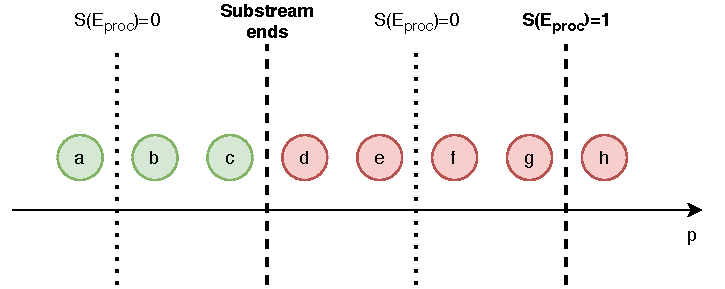
\includegraphics[width=0.50\textwidth]{pics/general-guarantee.pdf}
  \caption{Substreams management: general guarantee}
  \label{general_guarantees}
\end{figure}

A process can run this function on each new processing event to be informed when the substream has ended. Further, we say that function $S(E_{proc})$ provides a {\em notification} for an operator on the substream termination.

\subsubsection{Strict guarantee}

The guarantee that any new event will not satisfy the predicate is sufficient for many real-life problems, e.g., SPE can initiate process state pruning on such events. However, some problems require a more strict guarantee that the substream ends {\em exactly} after the last event. For example, epoch-based snapshotting protocol~\cite{2015arXiv150608603C, jacques2016consistent} requires notification that a process handles all elements from a specified epoch and nothing more to take the snapshot. If elements from different epochs are mixed, the snapshot can be inconsistent. To support such scenarios, function $S(E_{proc})$ should satsify the following condition:

\begin{align*}
& S(E_{proc}) = 1  \Longleftrightarrow \\
& \forall e^{'} = \langle proc,m,M_i\rangle, e^{'} >_p \sup E_{proc} : \neg pred(m), \\
& \sup E_{proc} = \inf_{e*} \forall e^{'} >_p e^{*} : \neg pred(m) 
\end{align*}

This condition allows a process to determine the exact moment (processing event) when the substream terminates: all elements after the notification will not satisfy the predicate, but all previous elements satisfy. Figure~\ref{strict_guarantees} illustrates the notion of the strict guarantee. As in the previous example, terms $a,b,c,d...$ denote ordered processing events of a process $p$. However, in this case, $S(E_{proc})=1$ right after the substream terminates and $S(E_{proc})=0$ for all previous events.

\begin{figure}[htbp]
  \centering
  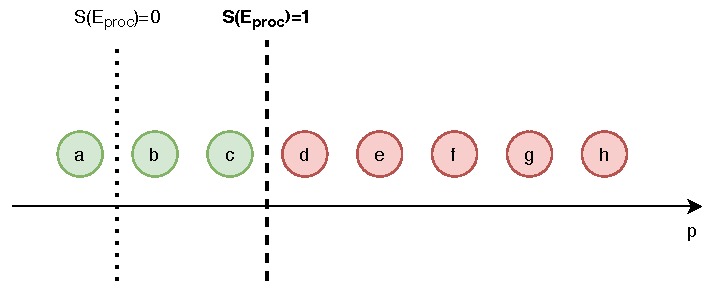
\includegraphics[width=0.50\textwidth]{pics/strict-guarantee.pdf}
  \caption{Substreams management: strict guarantee}
  \label{strict_guarantees}
\end{figure}

To implement such function in practice, it is often required to buffer input events until some condition is fulfilled. Therefore, one may need to define custom order of events processing $R(e)$ as well:

\begin{align*}
& R(e=\langle recv,m\rangle): R(e=\langle recv, x\rangle) > R(e=\langle recv, y\rangle) \\
& \Longleftrightarrow e=\langle proc,x,X_i\rangle >_p e=\langle proc,y,Y_i\rangle
\end{align*}

\subsubsection{Consistent notifications order}
Some specific applications, including the mentioned earlier epoch-based snapshotting method and techniques for enforcing deterministic processing~\cite{we2018adbis} require an order of notifications to be coincident with the order of substreams endings. For example, if notifications are reordered, then snapshots for consecutive epochs can be inconsistent.

\begin{figure}[htbp]
  \centering
  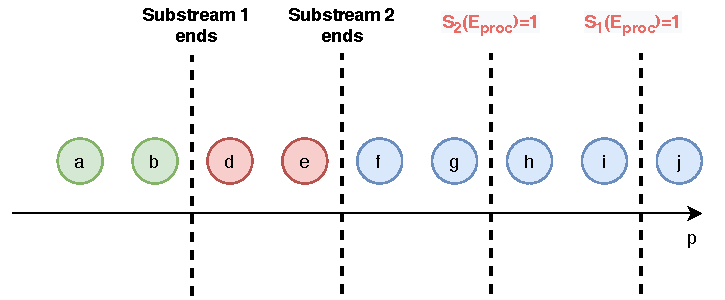
\includegraphics[width=0.50\textwidth]{pics/notifications-reordering.pdf}
  \caption{An example of notifications reordering}
  \label{notifications_reordering}
\end{figure}

Notifications reordering in case of the general guarantee is illustrated in Figure~\ref{notifications_reordering}. Terms $a,b,c,d...$ denote ordered processing events of a process $p$. Despite the fact that substream containing events $a,b$ terminates earlier, the notification function $S_1(E_{proc})$ for this substream detects termination after the notification function $S_2(E_{proc})$ for the substream containing events $d,e$. More formally, notification functions $S_1(E_{proc})$, $S_2(E_{proc})$ for corresponding substreams defined by predicates $pred_1(m)$, $pred_2(m)$ are {\em consistently ordered} iff:

\begin{align*}
& \forall E_{proc}: S_2(E_{proc})=1 \wedge S_1(E_{proc})=0 \Longrightarrow  \\
& \exists e=\langle proc, m, M_i\rangle > \sup E_{proc} : pred_1(m)
\end{align*}

\subsection{Punctuations framework}

\subsubsection{Framework overview}

The main idea behind the punctuations framework is to divide the stream into substreams by injection of special elements that bear predicate $pred(m)$. Punctuations are injected directly into a system as ordinary data elements by SPE or by external data producers. The injector promises that all further produced records do not satisfy the predicate. Hence, the punctuation itself defines the ``border'' of a substream.

Figure~\ref{punctuations_scheme} illustrates the punctuations framework. Green elements indicate elements which belong to some substream, while red elements do not. As we can see, punctuations play the role of delimiter between elements of the substream and all further items.

\begin{figure}[htbp]
  \centering
  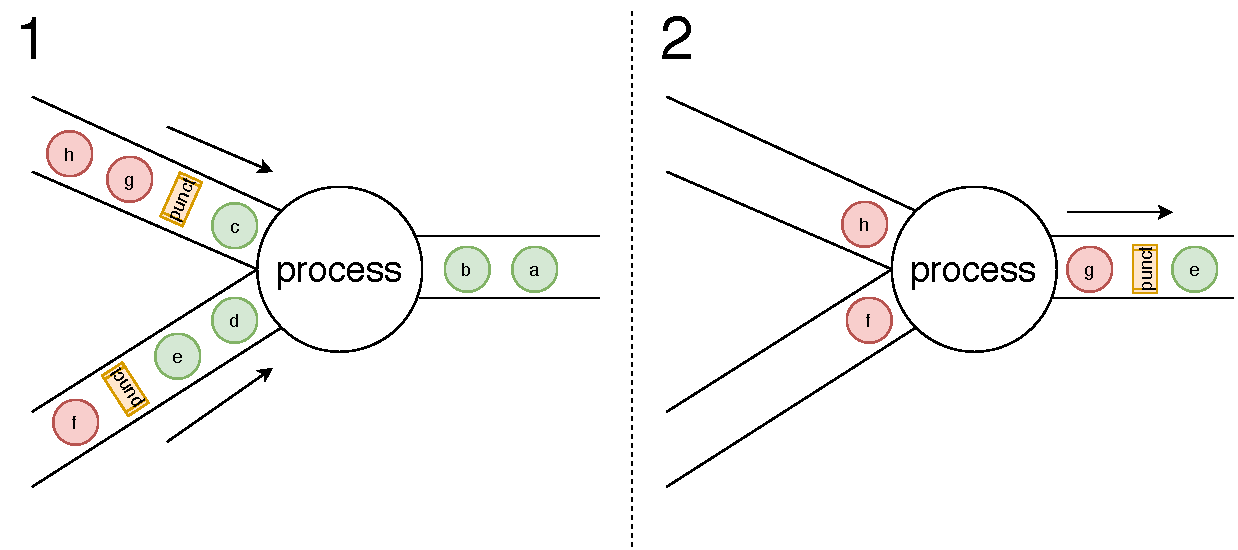
\includegraphics[width=0.50\textwidth]{pics/punctuations-scheme.pdf}
  \caption{Punctuations framework: an example}
  \label{punctuations_scheme}
\end{figure}

Processes withins SPE do not apply user-defined operators to punctuations. Instead, each process propogates a punctuation to all outgoing channels when it receives corresponding punctuations from all input channels. If a process receives punctuations from all inputs, it is guaranteed that it do not receive elements that satisfy the predicate further due to FIFO network channels. Therefore, function $S(E_{proc})$ for punctuations framework is the following:

\begin{align*}
& S_{punct}(E_{proc}) = \forall q \in I_p, \exists e \in E_{proc} : e = \langle recv,pred(m)\rangle_{qp}
\end{align*}

To make this function satisfy the strict notifications guarantee, one needs to block input channels which received punctuations until all other channels receive them. In~\cite{Carbone:2017:SMA:3137765.3137777} such behavior is called {\em watermark (punctuation) alignment}. The processing order function $R_{punct}(e)$ for this case should satisfy the following condition:

\begin{align*}
& \exists q \in I_p, e = \langle recv,m \rangle >_p e^{'} = \langle recv,pred(m)\rangle_{qp} \Longrightarrow \\ 
& R(e) > R(e^{*}= \langle recv,pred(m) \rangle_{q^{'}p}), \forall q^{'} \in I_p
\end{align*}

The punctuations framework provides consistent notification order by design because punctuations are naturally ordered with ordinary data elements within the processes. The formal proofs that function $S_{punct}(E_{proc})$ with the corresponding ordering satisfy general and strict guarantees as well as the proof that punctuations framework provides consistent notifications order are in the appendix~\ref{appendix:punctuations-proof}.

\subsubsection{Discussion}

While the punctuations approach is powerful and easy-to-implement, it has several limitations. In the punctuations framework, the information about the ending of a substream is propagated using ordinary data elements via the data flow network channels. It implies that punctuations are not applicable for cyclic dataflows because a process that receives elements from a cyclic channel will never receive punctuations from this channel~\cite{carbone2018scalable}.

The high network overhead forms another limitation. This method's amount of service traffic is $O(F||\Pi||^2)$, where $||\Pi||$ is the number of processes and $F$ is the frequency of punctuations injection. It is quadratic in the number of processes, as each process should propagate punctuations to all output channels. Such elements broadcasting may affect the throughput of an SPE. As we demonstrate further, the punctuation technique adds significant performance overhead on regular processing for small substreams (frequent punctuations injection).